% Define the scope, extend, and how of the study
\chapter{Methodology}
\label{chap:methodology}
% \begin{figure}
%   \centering
%   \graphicspath{ {../schemas/methodology/} }
%   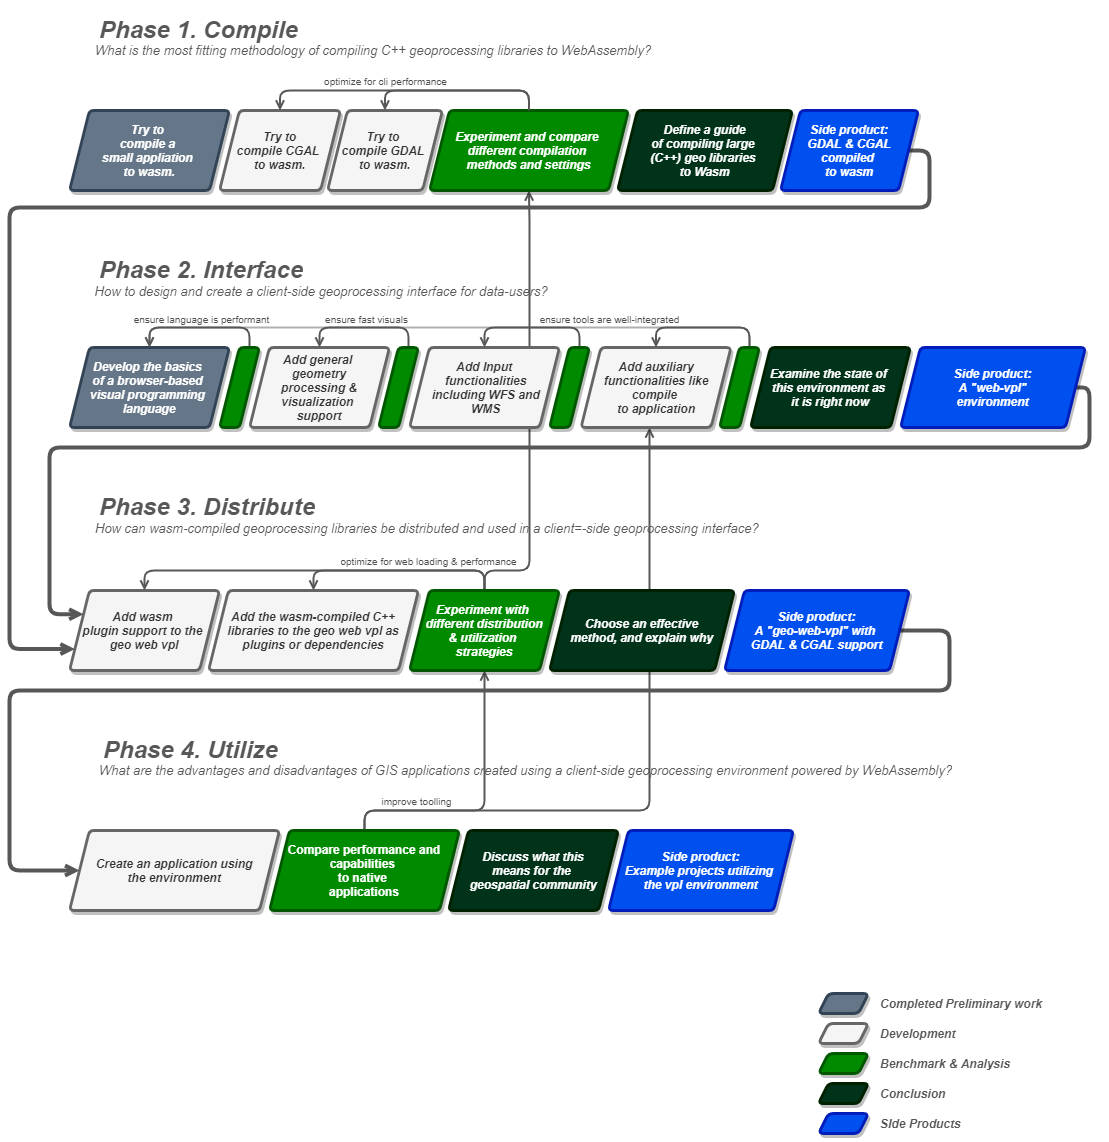
\includegraphics[width=14cm]{method.png}
%   \caption{Methodology schema}
%   \label{fig:method}
% \end{figure}

% The methodology used can be characterized as both incremental and iterative. Its incremental nature means that every phase, and every step within a phase, will produce meaningful in-between products \& results. This ensures the study will be insightful, even in the case the full scope of this study might become unfeasible. It is also vital for making the methodology iterative. 

% The study's iterative nature means that analysis and benchmarks will not be postponed until the end of the study, and will instead be an intricate part of each step. This makes sure obstacles are discovered early, and the trajectory of the study can be adjusted dynamically.  

% Every phase contains a number of development \& analysis steps. The reasoning behind these steps are covered by the following sub-chapters.

\subsubsection*{Overall Methodology}

\begin{note}
Choices: 
- practical > theoretical : Literature study indicates enough theoretical soundness, but lots of practical questions remaining. We wish to  immediate pick up where these studies have left, and therefore we choose the direct, practical study of designing and implementing a prototype application. 
- wholistic > specific    : Research in one sub-domain could have been more exhaustive in one of the specific sub-studies, instead of covering the full scope it does now. However, This would have been incomplete in a sense. What we do now is cover the full pipeline of using a geo-computation library: from creation to web export, to web import, to web utilization. by doing this, we can identify issues caused in one of these
- iterative > linear      : Given this vast scope, many questions can come up from different angles. The study has to be dynamic to adapt to these demands. 

Structure: 
- three sub-studies : sq1 tm 3
- the assessment : sq4

NOTE: I got the advice to explain less, to 'dig my own grave' less. I won't argue about these things, and just state them. But I do have my reasons

...
% Theorie: is er maar je geloofde het niet
% praktische implementatie om de Throerie weerleggen
The prior works on browser-based geoprocessing indicate that a theoretical framework for browser-based geoprocessing vpl is in place. 
But, and this is especially evident in the studies regarding client-side geoprocessing, the practical implementation of these theories

This necessitates a practical approach in response. 

, the advantages of a vpl, 
...
\end{note}

The methodology of this study can be characterized as practical as opposed to theoretical, wholistic instead of specific, and iterative compared to linear.
 
The methodology is subdivided into three sub-studies, based on the first three sub-research questions: \refsec{sec:method-one}, \refsec{sec:method-two}, and \refsec{sec:method-three}.  
These three studies are conducted to find answers to the major 'hows' of the geo-web-vpl. 
The literature was unable to provide answers with sufficient coverage, but did provide a strong starting point. 

While this may give the impression that these are separate, isolated issues, the design of one of these  questions was often presented by results from the two other components. 
The separation is made for narrative clarity, at the cost of accuracy. 

To properly examine the effectiveness of these 'hows' combined, experiments are conducted using the full extend of the solution. This is covered by the \refsec{sec:method-four} and final sub-research question.

%%%%%%%%%%%%%%%%%%%%%%%%%%%%%%%%%%%%%%%%%%%%%%%%%%%%%%%%%%%%%%%%%%%%%%%%%%%%%%%

\section{Problem Definition?}
% Inhibitors: 

Should I re-iterate the exact problem we are trying to solve? 

VPL
- Closed-source nature 
- Difficulty to integrate with 'regular' software

Browser-based geoprocessing
- Nature of geodata processing: 
  - Big data 
  - lots of IO operations (writing files away)

- Javascript:
  - different library ecosystem 
  - hard to utilize for geodata which requires a strongly typed environment 



\section{Sub Study 1: Web geo-computation libraries}
\label{sec:method-one}

\begin{note}
  Note that this is different from sub study 3.
\end{note}
\mySubRQOne

% not as easy 
% The study starts out with the assumption that WebAssembly must be utilized to properly compile and run existing geoprocessing libraries in a browser. This might not be as easy as using normal compilers, based on the experience gained by preliminary work (See \autoref{sec:preliminary-wasm}). WebAssembly is containerized and makes no assumptions about its source language \cite{haas_bringing_2017}, making aspects such as an SDK, sub-dependencies called using environment variables, and IO (file reading and writing) possible obstacles. These aspects might be solved by using or writing wrapper libraries and using file system workarounds, as proposed by \cite{jangda_not_2019}. 

% question & steps to answer
The first sub-question is dedicated to overcoming Obstacle 1, and uses the related works on \ac{wasm}. It goes: \textbf{"What is the most fitting methodology of compiling C++ geoprocessing libraries to WebAssembly?"}.
We specify ourselves to C++, since this seems to be the language of choice for almost all well established geoprocessing libraries. 
'Fitting' in this context refers to the specific requirements posed by geoprocessing libraries. 
The libraries are large and complex, and the geodata used as input even more so. 
This means special attention will be given to these aspects. 
Standard compiler effectiveness criteria, such as portability (smallest file size), and performance, will also be considerations during the assessment of methodologies.  

While the question poses to find the \textit{best} compilation method, if it turns out that only one method makes it possible to compile sizable geo-libraries, this phase will nonetheless regard itself as successful. The question will have to be rephrased in that case. 

% performance
\subsubsection*{Performance}
The performance benefit of WebAssembly is an important component of why WebAssembly might be beneficial for client-side geoprocessing. As such, this phase is interested in confirming whether this is the case for geoprocessing applications. Once a sufficient compilation method is found, individual functions of geoprocessing libraries will be benchmarked using three different methods: 

\begin{itemize}
  \item Compiled and run as native binary (g++), 
  \item Compiled to wasm, run natively (WASI),
  \item Compiled to asm.js, run natively (NODE.js),
\end{itemize}

% why cgal & GDAL
\subsubsection*{Test Cases}
CGAL \& GDAL will be used as examples of "C++ geoprocessing libraries" for this phase. For one, these libraries are well established and relevant to geoprocessing as a whole. Many other geo-libraries depend on them. Moreover, they are large and complex, making it highly likely the problems described by related works will be encountered. We could choose more simple libraries, but this will not be representative of most C++ geoprocessing libraries. 

While CGAL \& GDAL will be this phase's primary subject, the answer of this sub-question aims to be applicable to all geoprocessing libraries. 

%%%%%%%%%%%%%%%%%%%%%%%%%%%%%%%%%%%%%%%%%%%%%%%%%%%%%%%%%%%%%%%%%%%%%%%%%%%%%%%
%%%%%%%%%%%%%%%%%%%%%%%%%%%%%%%%%%%%%%%%%%%%%%%%%%%%%%%%%%%%%%%%%%%%%%%%%%%%%%%
%%%%%%%%%%%%%%%%%%%%%%%%%%%%%%%%%%%%%%%%%%%%%%%%%%%%%%%%%%%%%%%%%%%%%%%%%%%%%%%
%%%%%%%%%%%%%%%%%%%%%%%%%%%%%%%%%%%%%%%%%%%%%%%%%%%%%%%%%%%%%%%%%%%%%%%%%%%%%%%
%%%%%%%%%%%%%%%%%%%%%%%%%%%%%%%%%%%%%%%%%%%%%%%%%%%%%%%%%%%%%%%%%%%%%%%%%%%%%%%

\section{Sub Study 2: Application \& Interface}
\label{sec:method-two}

\mySubRQTwo

% We ask ourselves if the current state of client-side web technologies are capable of facilitating multiple steps of geodata conversion, and what such an application would look like. 

Phase 2 is dedicated to overcoming Obstacle 2, assisted by the related works on the geoweb. Phase 2 seeks to not only make geoprocessing runnable, but actually usable, and usable to a wide audience of "data-users". This quest is posed using the research question: \textbf{How to design and create a client-side geoprocessing environment for data-users?}. 

Phase 2 will primarily be about implementing the foundations of the use-case application 'GeoFront'. None of the existing web-based \ac{vpl}'s were deemed acceptable for the scope of this study, so the application will have to be created from scratch. 
The application will be created using JavaScript, or its type-save equivalent TypeScript. 
A choice can be made to write the whole environment as a native application which then, as a whole, can be published to the web using WebAssembly. 
This would probably be the most performant. 
However, referring back to the FAIR principles of \cite{mark_d_wilkinson_fair_2016}, this would be detrimental to the concept of Interoperability and Reusability. 
We wish the environment to contain small, standalone components which could be useful in and of themselves. 
For example, users might want to integrate a geodata process on their own website without the full \ac{gui} attached.

The modern web contains many technologies we can possibly use to facilitate all required features. WebGL offers the ability to efficiently visualize 3D data. The 2d canvas API and SVG's can be used to visualize 2D data. HTML can be used to build the interface.

\subsubsection*{Steps}

Just like the entire study, the development trajectory during phase 2 will be done incrementally, ensuring results can be shown during all steps of the development. 
The first step of the phase will consist of creating the basics of the \ac{gui} itself. a basic \ac{vpl} will be created which can only process boolean statements. The second step adds types, geometry, and the visualization of this geometry in 3D, as well as textures / images in 2d. The third step will add geospatial data support, like Web Feature Services, Web Map Services, and coordinate reference systems.  

%%%%%%%%%%%%%%%%%%%%%%%%%%%%%%%%%%%%%%%%%%%%%%%%%%%%%%%%%%%%%%%%%%%%%%%%%%%%%%%
%%%%%%%%%%%%%%%%%%%%%%%%%%%%%%%%%%%%%%%%%%%%%%%%%%%%%%%%%%%%%%%%%%%%%%%%%%%%%%%
%%%%%%%%%%%%%%%%%%%%%%%%%%%%%%%%%%%%%%%%%%%%%%%%%%%%%%%%%%%%%%%%%%%%%%%%%%%%%%%
%%%%%%%%%%%%%%%%%%%%%%%%%%%%%%%%%%%%%%%%%%%%%%%%%%%%%%%%%%%%%%%%%%%%%%%%%%%%%%%
%%%%%%%%%%%%%%%%%%%%%%%%%%%%%%%%%%%%%%%%%%%%%%%%%%%%%%%%%%%%%%%%%%%%%%%%%%%%%%%

\section{Sub Study 3: Direct Utilization}
\label{sec:method-three}
\mySubRQThree


% \section{Proposed Model}

% (a diagram showing relationships between vpl, libraries, javascript, webassembly)

% - javascript-subset library wrappers 
%   - 
%   -
%   - magic methods

% - different javascript-subset for vpl runtimes 



% performant and sharable geoprocessing
% portability


The third phase is characterized by harmonizing the results of Phase 1 and 2. 
The related works pointed out that WebAssembly can only truly be tested within a realistic use-case scenario, So this Phase intends to do just that.
The research question goes: \textbf{What is the best way of distributing wasm-compiled geoprocessing libraries, in order to use them within a client-side geoprocessing environment?}. 
This phase can be seen as a continuation of phase 1, but where the compilation research of phase 1 limits itself to native, CLI usage of WebAssembly, this phase introduces the web, and the developed interface during phase 2 as new factors to this research. Given this as the desired way of processing geodata, how can WebAssembly facilitate these desires? 

This will result in new benchmarks, and new analyses, now including factors like client-side (down)load times, compilation, and utilization. Answers will have to be given to questions such as \textit{Where do the wasm-compiled libraries live?} and \textit{ how are they cached? }.

% One of the hypothetical obstacles during this phase is that an entire geoprocessing library will have to be downloaded, even if the user desires only a single function. A solution to this problem is to increase granularity, and split up the C++ libraries to several smaller ones, maybe even one wasm binary per function or class. This would be accompanied by WebAssemblies ability to accept \ac{wasm} dependencies at the time it is loaded into memory. 

%%%%%%%%%%%%%%%%%%%%%%%%%%%%%%%%%%%%%%%%%%%%%%%%%%%%%%%%%%%%%%%%%%%%%%%%%%%%%%%
%%%%%%%%%%%%%%%%%%%%%%%%%%%%%%%%%%%%%%%%%%%%%%%%%%%%%%%%%%%%%%%%%%%%%%%%%%%%%%%
%%%%%%%%%%%%%%%%%%%%%%%%%%%%%%%%%%%%%%%%%%%%%%%%%%%%%%%%%%%%%%%%%%%%%%%%%%%%%%%
%%%%%%%%%%%%%%%%%%%%%%%%%%%%%%%%%%%%%%%%%%%%%%%%%%%%%%%%%%%%%%%%%%%%%%%%%%%%%%%
%%%%%%%%%%%%%%%%%%%%%%%%%%%%%%%%%%%%%%%%%%%%%%%%%%%%%%%%%%%%%%%%%%%%%%%%%%%%%%%

\section{Assessment}
\label{sec:method-four}
\mySubRQFour

\begin{note}
  - todo: turn features around into assessment criteria
\end{note}

Finally, When the VPL contains all tools necessary to be used to properly process geodata, a final assessment can be made by using the environment to serve as an application. this assessment will try to overcome Obstacle 3 by posing the question: \textbf{What are the advantages and disadvantages of GIS applications created using a client-side geoprocessing environment powered by WebAssembly?}. This question requires a native but comparable GIS application to test this against.  

We hypothesize that applications equipped with client-side geoprocessing open up a whole range of new possibilities posing both academic \& commercial benefits. 
These aspects of the study can be discussed during this phase. 




\section*{Features}

\emph{Q: Which features are required for a 'usable' VPL intended for geo-computation?}

We define three major features.  

These features are in turn based upon related works within VPL research, as well as web GIS studies. 
This section outlines these requirements, and explains why they are used. 
Additionally, certain use-cases are envisioned as proxies of these requirements, to test certain requirements in a realistic scenario. 

...

\subsection*{Feature A: Interactive}

A VPL should be Interactive.

\begin{lstlisting}



  Interactivity is the defining factor of the vpl. 
  a list of standard VPL features & application features required as a base-line:  
- Users must be able to construct a script by visual means.
- Dataflow Modelling
- Dragging and dropping is a ui which

(geo-vpl features:)
- read data from user-submitted files
- write data to files, downloadable by the user  
- debug / inspect data in a 3D viewer
- draw geometry in a 3D viewer

\end{lstlisting}





% NOTE: these are the '1 or 2 major contributions, besides making a web-geo-vpl'
\subsection*{Feature B: Extendable}

A VPL should be Extendable. 

\begin{lstlisting}
REASON: 
  - VPL: Important take away from meta-analysis: extendability
  - WEB: Geoweb: FAIR principles -> fair geoprocessing

CRITERIA
  - ease of creating and using plugins 
  - ease of using existing geo-libraries 
  - written in non-js languages

  The quality of plugin creation and utilization
The extend in which existing, non-js, industry-standard libraries can be used

\end{lstlisting}



\subsection*{Feature C: Publicability (the ability to publish / operationalize) } 

A VPL should be Publicable. What is meant by that, is that scripts designed by using the VPL should be 

\begin{lstlisting}

REASON: 
 - VPL: application life-cycle is important: how to publish & use applications created using vpl's
 - WEB: cloud-native geoprocessing: requires server-side / cloud based
   geo-computation interoperability: 
   meaning the scripts must be able to be used without any of the 
   interactivity features.

CRITERIA:
 - ease of sharing apps as a visual program
 - ease of compiling and running the app headless
\end{lstlisting}



\section{Evaluation}

\emph{Q: Usage: Who benefits from a web-geo-vpl, and how?  }

A web-based visual programming language for geo-computation as described by this study does not exist yet. 
This requires us to be clear about its intended use-case. 
However, because of this same novelty, a singular, definitive use-case can not be given.
To solve this problem, this study names four possible use-cases.  
These cases are not mutually exclusive, but will be judged separately, based on specific criteria 
During assessment, we will use these four profiles and accompanying criteria to judge how well the geo-web-vpl meets up this use-case.

\subsection*{Case 1: Educational Sandbox}

"
insight within these processes are vital for communication, voor 'overdracht' 
the 'jonathan blow educational argument' 
"

- This use-case can be fully realized within the current state of geofront
- "Geoprocessing for kids"
- "What is a delaunay triangulation?" 
- "Let people play / experience / traverse a nef polyhedron"
- Using something helps with understanding

\subsubsection*{Criteria}
Used primairly as a test for \textbf{Criterium A}.


\subsection*{Case 2: Web Demo Environment}
% # A: 1. Geofront as a geoprocessing / analysis demo tool.
% - Frame Geofront as an expanded version of https://validator.cityjson.org/ this. 
%   - [this](https://validator.cityjson.org/) (a wasm web demo) + jsfiddle 
%   - Use rust, web, and c++ tools side by side, hand in hand

- Reproducibility toolkit:
- Workflow: 
  - Load your own code from a CDN
  - Build a demo setup around it
  - load a custom graph from a public json file
  - share a url pointing to this json (which contains the CDN address)
- You can now share a rust / C++ program as a fully usable web demo,   
  and analyze its performance using different datasets, test parameters, etc. 
- interdisciplinary exchange of ideas
- MISSING FEATURE: dependency list inside of the graph.json save file

% Within the field of geo-informatics, we want to share our end-results. 
% - Usually on git, but this has limitations:
%     - Not everybody can immediately use it ( unfamiliar language / build system),
%     - Even people who can understand, often wont go through the trouble.  
%     - "Python bindings" -> half-solves the problem, but still hard to publish to a general audience. 

% This was the exact reason for developing https://validator.cityjson.org/. This solved the issue of publication. Why? 
% - Extremely findable, usable, accessible
%   - Cross-platform
%   - No install 
%   - first point of contact is precisely where you can use it
%   - You can send a link not to a download page, but to the application itself
%   - Great for communication: blogs with embedded applications.
%   - Code sharing: you exactly know what to expect.

\subsubsection*{Criteria}
Used primairly as a test for \textbf{Criterium B}.
show that criteria B can be used to strip down the environment to purely that which needs to be demonstrated.

\subsection*{Case 3: End User Geoprocessing Environment}
- Lightweight FME, but open source \& on the web.
- The tool in itself can be regarded as an end-user application:
  - Load file, do something with the file, download resulting file
  - REQUIRES WAY MORE SUPPORTING LIBRARIES AND TOOLS
- Flowcharts can be exchanged by means of url's.
- Future work: export flowchart to a process which can be run natively or server side.
  

\subsubsection*{Criteria}
Used primairly as a test for \textbf{Criterium C}.


\subsection*{Case 4: Rapid-Prototyping Environment}
\begin{lstlisting}
- Web geoflow
- To be used within a regular software development process.
- Ravi's GeoFlow, but on the web
- Meant to visually debug a certain process, after which this process can be 'compiled' to a normal cli tool.


  WHY: 
  - all three the previous use-cases combined: demo, test, educate yourself
    on your own algorithms, then operationalize the code to use it in a 
    serious environment.  

  
\end{lstlisting}





% - CURRENTLY MISSING FEATURE: compile to native cli tool (node.js script)
% - REQUIRES WAY MORE SUPPORTING LIBRARIES AND TOOLS


\subsubsection*{Criteria}
A total test of \textbf{Criteria A, B and C}.


% <br><br>

% ## Web Demo & Scripting environments

% we are not the first to recognize the suitability of the web for publishing demo's

% We see a lot of interactive web-demo's nowadays, and many of them are embedded within a type of "Demo Hosts":

% - Scripting environments in (Science) Communication:
%   - Jupyter Notebook 
%   - Observable
%   - JsFiddle
%   - Shadertoy
%   - Wapm

% - Scripting environments in Education: 
%   - TU Delft C++ course
%   - Udemy

% - Scripting environments in Tutorials: 
%   - Rust
%   - Lit

%   <!-- - (game-jam games)
%       - more save (no virus) -->

% <!-- We also see 

% - As accessible alternative to native
%   - Overleaf -> does not use webassembly, but a classic client-server architecture
%   - Google Earth -->

% All these applications lie on a crossroad between being an interactive demonstration of a certain result or phenomenon, 
% and an open invitation for the user to edit and use this result or phenomenon. 
% (CITE A STUDY PROVING HOW INTERACTION BENEFITS LEARNING), 
% so toying around is important.

% <!-- So it is save to say the web is suitable for these types of things. 
% But is the web also suitable for more? Can we use a web-based sandbox environment to -->


% we want to examine and edit the geodata flow, see for example, where these errors occur, try to get to that data, see if we can make hotfixes, etc. etc. 
